
We monitored the accuracy of our embeddings over the course of training our CNN. The validation set is a dataset of 1000 triplets such that 100 triplets are created from each of the 10 validation videos. After the end of training, 736/1000 samples fulfilled the triplet constraint. 930/1000 fulfilled the contrained without the added margin. I.e. $\norm{x_a - x_p} < \norm{x_a - x_n}$.

For comparison after 10 epochs of training the values were 467/1000 with margin and 894/1000 without the margin.

{
    \centering
    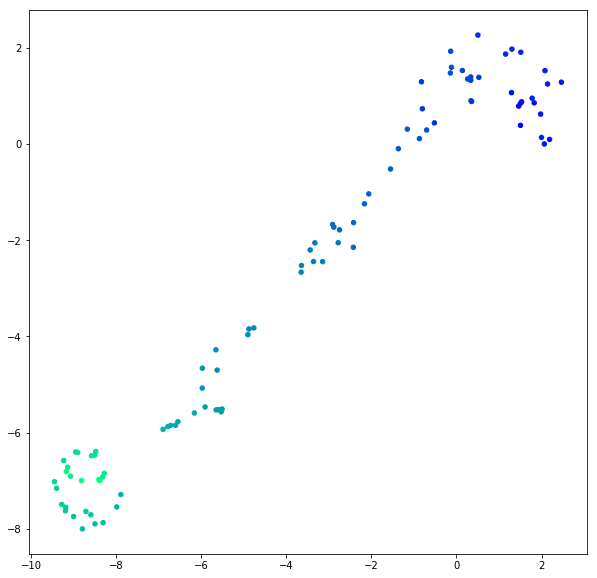
\includegraphics[width=8cm]{t-sne-trajectory.png}
    \captionof{figure}{A t-SNE plot of a validation trajectory. Perplexity 30, learning rate 200 and 1000 iterations. The color goes from blue to cyan as a function of the frame indices.}
    \label{t-sne}
    \vspace{0.25cm}
}

The t-SNE plot in figure \ref{t-sne} of a validation trajectory suggests that the network has learned a meaningful and well-behaved embedding of the video frames. Embeddings of frames that are close to each other in the video are close to each other in the dimensionality reduced regime.

{
    \centering
    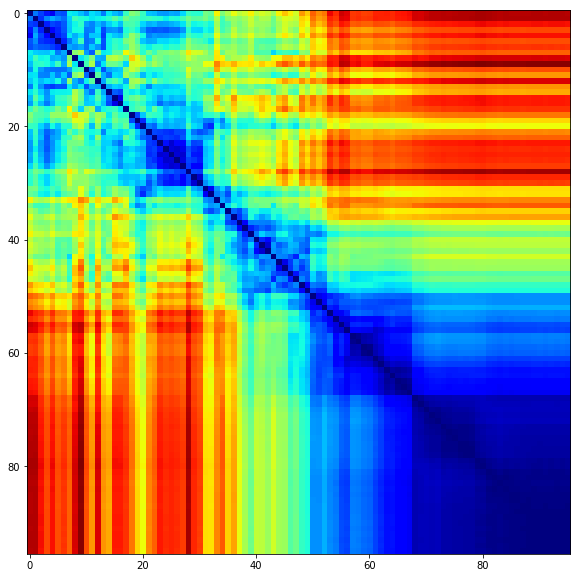
\includegraphics[width=8cm]{dima.png}
    \captionof{figure}{Visualization of the $L_2$ distance matrix of the same validation video as in figure \ref{t-sne}. Blue means close and red is far away.}
    \label{dima}
    \vspace{0.25cm}
}

{
    \centering
    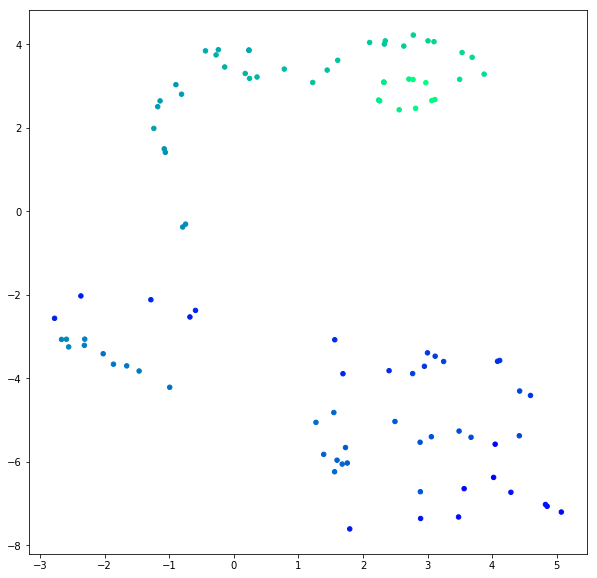
\includegraphics[width=8cm]{early_trajectory.png}
    \captionof{figure}{For comparison, a visualization of a trajectory after 50 epochs of training. Visualized using the same t-SNE parameters and the same video as figure \ref{t-sne}.}
    \label{early-t-sne}
    \vspace{0.25cm}
}
{
    \centering
    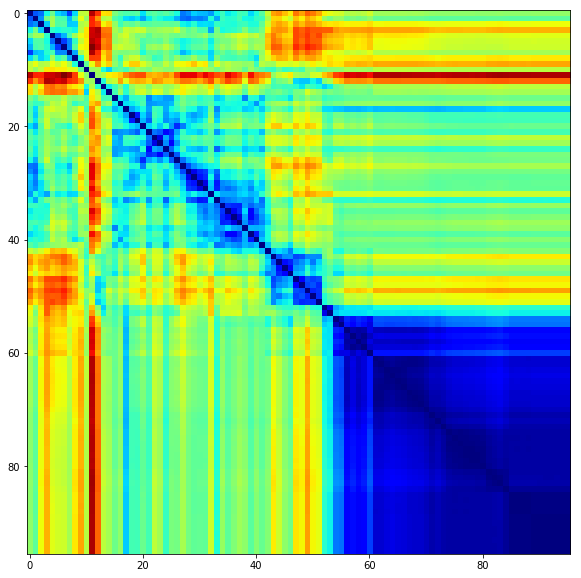
\includegraphics[width=8cm]{early-dima.png}
    \captionof{figure}{Distance matrix for the same network as in figure \ref{early-t-sne}.}
    \label{early-dima}
    \vspace{0.25cm}
}

Each row and column in the distance matrix shown in figure \ref{dima} corresponds to a frame of the video. The value is the euclidean distance between the embedding of the frame. I.e. the diagonal is 0 and the matrix is symmetric. This visualization seems to confirm that subsequent frames are close to each other in the embedding space.

Comparing figure \ref{t-sne} to figure \ref{early-t-sne} and figure \ref{dima} to figure \ref{early-dima} we can see that early on in training the network has not yet learned a meaningful embedding of the entire joint space of the robot.

